\section{增大和减小摩擦的方法}\label{sec:3-12}

实验研究表明,摩擦力随着压力增大而增大,还跟接触面的粗糙程度有关系,接触面越粗糙,摩擦力越大。
我们有了这些知识,就能够在摩擦对我们有益的场合想办法来增大它。

摩擦力随着压力增大而增大,所以增大压力可以增大摩镲。
在皮带传动(图 \ref{fig:3-13})中,皮带和皮带轮之间的摩小了,皮带就会在皮带轮上打滑,不能带动机器正常运转。
遇到这种情况可以张紧皮带,增大皮带对皮带轮的压力,来增大它们之间的摩擦。
我们要拿起一个很重的东西,就要用劲捏紧它,这是因为用劲捏可以增大手对重物的压力,也就增大了它们之间的摩擦力,
摩擦力足够大时,重物就不会从手中滑掉。

\begin{figure}[htbp]
    \centering
    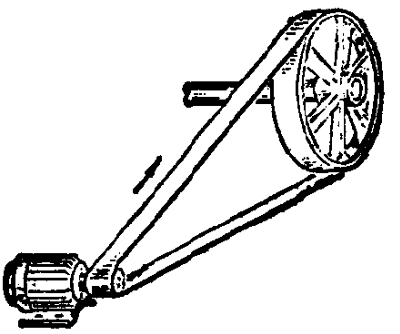
\includegraphics[width=0.3\textwidth]{../pic/czwl1-ch3-13}
    \caption{皮带传动}\label{fig:3-13}
\end{figure}

接触面越粗糙,摩擦就越大,所以把接触面弄得粗糙些可以增大摩擦。
自行车、汽车、拖拉机的轮胎表面有凹凸的花纹,就是为了把接触面弄得粗糙些来增大摩擦,
使刹车时轮胎滑行较短的距离就可以停下,开车时轮胎不致在原地打滑。
在北方的冬季,铁轨上往往结一层薄冰,机车车轮跟铁轨的摩擦变得很小,机车开动了,但车轮只是在铁轨上滑转,
列车不能前进。这时如果在铁轨上撒些沙子来增大摩擦,列车就可以前进了。

机器内部有许多转动部分和滑动部分,运转的时候都有摩擦,这时摩擦不但使机器发热,白白消耗动力,
而且会使机器磨损,性能变坏,在这些场合摩擦是有害的,应该设法减小摩擦。

在机器内部的转动部分都有轴和安装轴的轴承。
轴承分滑动轴承和滚动轴承两种,图 \ref{fig:3-14} 是滑动轴承,机器运转时轴和轴瓦间发生滑动摩擦。
图 \ref{fig:3-15} 是滚动轴承,轴承的内圈紧套在轴上,外圈固定在轴承座上,两圈之间装有许多光滑的钢珠或钢柱。
机器运转时,轴带着内圈转动,钢珠或钢柱在两圈之间动,摩擦就减小多了。

\begin{figure}[htbp]
    \centering
    \begin{minipage}{4cm}
    \centering
    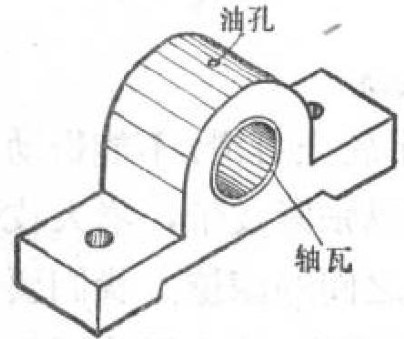
\includegraphics[width=4cm]{../pic/czwl1-ch3-14}
    \caption{}\label{fig:3-14}
    \end{minipage}
    \qquad \hspace{5em}
    \begin{minipage}{5cm}
    \centering
    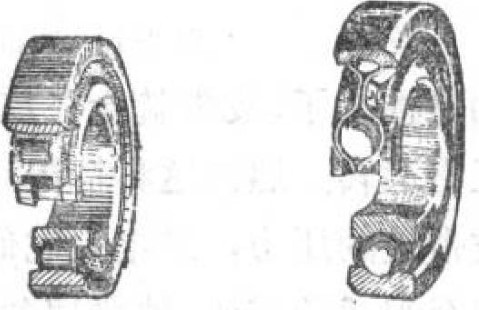
\includegraphics[width=5cm]{../pic/czwl1-ch3-15}
    \caption{}\label{fig:3-15}
    \end{minipage}
\end{figure}

由于滚动摩擦比滑动摩擦小得多,滚动轴承的摩擦大约是滑动轴承的摩擦的 $\dfrac{1}{20}$ ~ $\dfrac{1}{30}$,
所以机器的转动部分多安装滚动轴承。不过由于滚动轴承不能承受太大的压力,在很多场合还必须使用滑动轴承。
加润滑油可以在摩擦表面间形成油膜,使摩表面的凹凸部分不互相啮合,能够减小摩擦。
一般说来,加润滑油可以使摩擦减小到 $\dfrac{1}{8}$ ~ $\dfrac{1}{10}$。
良好的润滑是保证机器正常工作的不可缺少的重要条件。
机器的滑动轴承、滚动轴承以及其他运动部分,在运转时都必须得到良好的润滑。
润滑良好可以延长机器的使用年限,润滑不良,零件就磨损得快,我们在使用机器的时候,一定要注意润滑。


\lianxi

(1) 有些地区的公路,在冬季由于积有冰雪而变得很滑。汽车在这种公路上行驶,常常要在车轮上缠铁链。为什么?

(2) 克丝钳口上刻有花纹,这起什么作用?

(3) 犁的表面须保持光滑,为什么?用生锈的犁来耕地,有什么不好?

(4) 自行车上哪些地方要利用摩擦?哪些地方要减小摩擦?是用什么方法来增大和减小摩擦的?

(5) 在什么机器上你看到过滑动轴承?在什么机器上你看到过滚动轴承?它们是怎样润滑的?

(6) 你曾经遇到过哪些有益的摩擦和有害的摩擦?你能不能利用所学知识,提出增大有益摩擦和减小有害摩擦的建议?



\nonumsection{小实验:筷手提米}

\begin{wrapfigure}[11]{r}{4cm}
    \centering
    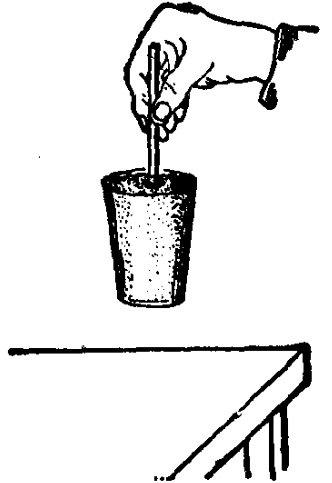
\includegraphics[width=4cm]{../pic/czwl1-ch3-16}
    \caption{}\label{fig:3-16}
\end{wrapfigure}

在一个玻璃杯里装上半杯大米,把一根筷子插在中间,将米压紧,使筷子直立。
然后陆续往杯子里加大米,一边加一边压紧,直到杯子里装满大米,然后往杯子里加少许水,
等一会儿,拿住筷子就可以把装满大米的玻璃杯提起来(图 \ref{fig:3-16})。
自己做做看,并想一想这是什么道理。


